% Agent n-gram transition score -- one-page idea note, in the style of ../tutorial/conftr-factuality.tex.
% Build: ./build.sh ngram  (pdflatex, output ngram.pdf)
\documentclass[10pt,a4paper]{article}
\usepackage[margin=1.4cm,top=1.1cm,bottom=1.0cm]{geometry}
\usepackage[T1]{fontenc}
\usepackage[utf8]{inputenc}
\usepackage{amsmath,amssymb}
\usepackage{xcolor}
\usepackage{framed}
\usepackage{tikz}
\usetikzlibrary{arrows.meta,backgrounds,calc}
\usepackage[hidelinks]{hyperref}
% Shared colours and boxes for tutorial.tex and cheatsheet.tex.
% Needs: xcolor, framed. (tcolorbox is not available in this TeX install.)

% ---------- palette ----------
\definecolor{secblue}{rgb}{0.10,0.22,0.48}
\definecolor{thmbg}{rgb}{0.93,0.95,1.00}   \definecolor{thmfr}{rgb}{0.20,0.33,0.68}
\definecolor{defbg}{rgb}{0.93,0.98,0.97}   \definecolor{deffr}{rgb}{0.05,0.45,0.42}
\definecolor{keybg}{rgb}{1.00,0.97,0.86}   \definecolor{keyfr}{rgb}{0.72,0.50,0.02}
\definecolor{recbg}{rgb}{0.94,0.96,0.98}   \definecolor{recfr}{rgb}{0.25,0.35,0.45}
\definecolor{clmbg}{rgb}{0.96,0.93,1.00}   \definecolor{clmfr}{rgb}{0.42,0.22,0.62}
\definecolor{ourbg}{rgb}{0.96,0.96,0.96}   \definecolor{ourfr}{rgb}{0.35,0.35,0.35}
\definecolor{okbg}{rgb}{0.92,0.98,0.92}    \definecolor{okfr}{rgb}{0.12,0.50,0.18}
\definecolor{nobg}{rgb}{1.00,0.93,0.92}    \definecolor{nofr}{rgb}{0.70,0.16,0.12}
\definecolor{codebg}{rgb}{0.965,0.965,0.955}
\definecolor{shadecolor}{rgb}{0.965,0.965,0.955}

% ---------- generic breakable colour box: \begin{cbox}[title]{background}{frame} ----------
\newenvironment{cbox}[3][]{%
  \def\FrameCommand{\fboxsep=7pt\fboxrule=0.9pt\fcolorbox{#3}{#2}}%
  \MakeFramed{\advance\hsize-\width\FrameRestore}%
  \if\relax\detokenize{#1}\relax\else
    {\noindent\textcolor{#3}{\sffamily\bfseries #1}\par\nobreak\vspace{3pt}}%
  \fi\noindent\ignorespaces}
 {\endMakeFramed}

% ---------- named boxes ----------
\newenvironment{keybox}[1][Key point]{\cbox[#1]{keybg}{keyfr}}{\endcbox}                 % take-aways
\newenvironment{recipebox}[1][Recipe]{\cbox[#1]{recbg}{recfr}}{\endcbox}                 % procedures
\newenvironment{claimbox}[1][Claims of the paper]{\cbox[#1]{clmbg}{clmfr}}{\endcbox}     % what a paper asks and claims
\newenvironment{oursbox}[1][Our reading]{\cbox[#1]{ourbg}{ourfr}}{\endcbox}              % remarks that are not the paper's
\newenvironment{okbox}[1][Guaranteed]{\cbox[#1]{okbg}{okfr}}{\endcbox}                   % what holds
\newenvironment{nobox}[1][Not guaranteed]{\cbox[#1]{nobg}{nofr}}{\endcbox}               % what does not
\newenvironment{thmbox}{\cbox{thmbg}{thmfr}}{\endcbox}
\newenvironment{defbox}{\cbox{defbg}{deffr}}{\endcbox}

% ---------- inline highlights ----------
\newcommand{\hl}[1]{\textcolor{secblue}{\textbf{#1}}}                    % key term
\newcommand{\yes}[1]{\textcolor{okfr}{\textbf{#1}}}
\newcommand{\no}[1]{\textcolor{nofr}{\textbf{#1}}}
\newcommand{\ctag}[1]{{\fboxsep=1.5pt\colorbox{clmfr}{\textcolor{white}{\sffamily\bfseries\scriptsize #1}}}}  % claim id
\newcommand{\kind}[1]{\textcolor{clmfr}{\textsf{\scriptsize[#1]}}}       % kind of claim


% ---------- notation ----------
\newcommand{\Dref}{D_{\rm ref}}
\newcommand{\R}{\mathcal{R}}
\newcommand{\bos}{\langle\mathrm{s}\rangle}
\newcommand{\norm}[1]{\lVert #1\rVert}

% ---------- line badges: the same number marks a line in the figure, the algorithm and the text ----------
\tikzset{badge/.style={circle,fill=recfr,text=white,inner sep=0.6pt,minimum size=9pt,font=\sffamily\bfseries\fontsize{6}{6}\selectfont}}
\newcommand{\lb}[1]{\tikz[baseline=(b.base)]\node[badge](b){#1};}

% ---------- pseudocode: one \al per line, optional argument = indent in em ----------
\newcounter{algline}
\newenvironment{algo}{\begin{list}{}{\setlength{\leftmargin}{1.7em}\setlength{\labelwidth}{1.2em}\setlength{\labelsep}{0.5em}%
  \setlength{\itemsep}{2pt}\setlength{\parsep}{0pt}\setlength{\topsep}{2pt}\setlength{\partopsep}{0pt}}}{\end{list}}
\newcommand{\al}[1][0]{\stepcounter{algline}\item[\lb{\arabic{algline}}]\hspace*{#1em}\ignorespaces}
\newcommand{\kw}[1]{\textbf{#1}}
\newcommand{\cm}[1]{\hfill\textcolor{ourfr}{\scriptsize\itshape #1}}
\newcommand{\algin}[1]{\noindent\textcolor{recfr}{\textbf{Input:}} #1\par}

% ---------- step cells for the figure ----------
\newcommand{\stp}[3]{{\fboxsep=1.3pt\fboxrule=0.4pt\fcolorbox{#1}{#2}{\tiny\strut$s_{#3}$}}}
\newcommand{\sany}[1]{\stp{recfr}{white}{#1}}
\newcommand{\slow}[1]{\stp{okfr}{okbg}{#1}}
\newcommand{\shigh}[1]{\stp{nofr}{nobg}{#1}}

\pagestyle{empty}
\setlength{\parindent}{0pt}
\setlength{\parskip}{3pt}

\begin{document}
{\Large\bfseries\color{secblue} An agent $n$-gram transition score for step suspiciousness}\\[1pt]
{\small\textcolor{ourfr}{A label-free step scorer: a step is suspicious when it moves unlike other steps under the same agent pattern. Idea note, untested.}}

\vspace{2pt}
\textbf{Setting.} A trajectory is $x=(s_1,\dots,s_T)$ and $a_t=A(s_t)$ is the agent responsible for step $t$. A frozen proxy encoder $\phi$ reads the whole trajectory and returns one vector per step, $e_1,\dots,e_T\in\mathbb{R}^d$. The \emph{movement} into step $t$ is $d_t=e_t-e_{t-1}$, with $e_0=0$. The \emph{key of order $j$} of step $t$ is the pattern of its last $j$ agents, $k_t^{(j)}=(a_{t-j+1},\dots,a_t)$ for $j=0,\dots,n$, where $a_t=\bos$ (a start symbol) for $t\le0$ and $k_t^{(0)}$ is the empty key shared by all steps. \textbf{Assumption:} most steps are correct, and a correct hand-off between the same agents moves in a similar direction each time.

\vspace{3pt}
\begin{center}
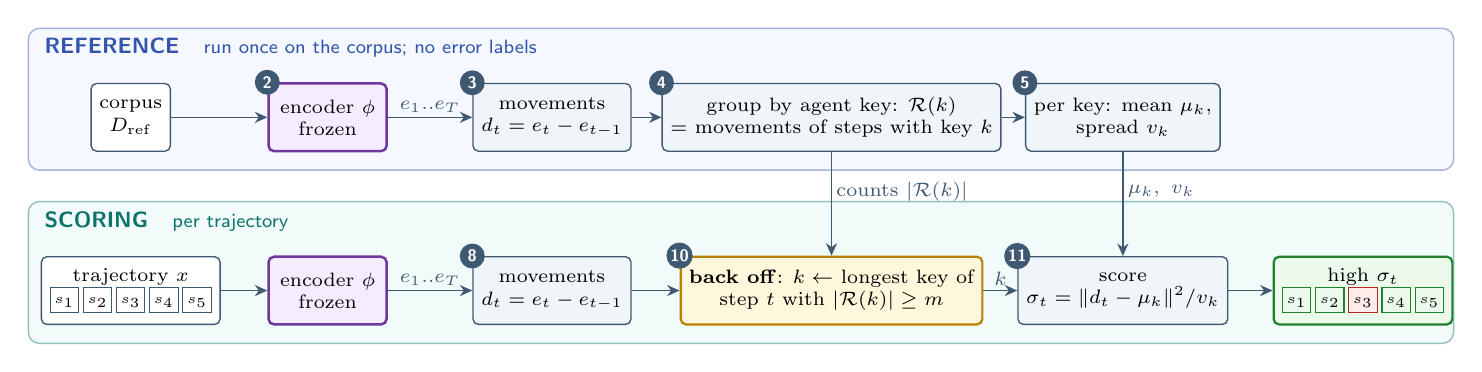
\begin{tikzpicture}[x=1cm,y=1cm,font=\scriptsize,%
  >={Stealth[length=4.5pt,width=4pt]},
  box/.style={draw=recfr,fill=white,rounded corners=2pt,align=center,inner sep=3pt,minimum height=0.86cm,line width=0.5pt},
  op/.style={box,fill=recbg},
  model/.style={box,draw=clmfr,fill=clmbg,line width=0.9pt,minimum width=1.5cm},
  soft/.style={box,draw=keyfr,fill=keybg,line width=0.8pt},
  good/.style={box,draw=okfr,fill=okbg,line width=0.8pt},
  flow/.style={->,draw=recfr,line width=0.6pt},
  lab/.style={font=\scriptsize,text=recfr,inner sep=1.5pt},
  ttl/.style={font=\sffamily\bfseries\footnotesize,anchor=west,inner sep=0pt}]

% ================= reference band =================
\node[ttl,text=thmfr] at (-0.05,0.33) {REFERENCE\quad{\normalfont\sffamily\scriptsize run once on the corpus; no error labels}};
\node[box] (dr) at (1.05,-0.55) {corpus\\$\Dref$};
\node[model] (e1) at (3.55,-0.55) {encoder $\phi$\\frozen};
\node[op] (m1) at (6.40,-0.55) {movements\\$d_t=e_t-e_{t-1}$};
\node[op] (gr) at (9.95,-0.55) {group by agent key: $\R(k)$\\= movements of steps with key $k$};
\node[op] (st) at (13.65,-0.55) {per key: mean $\mu_k$,\\spread $v_k$};

\draw[flow] (dr.east) -- (e1.west);
\draw[flow] (e1.east) -- node[lab,above]{$e_1..e_T$} (m1.west);
\draw[flow] (m1.east) -- (gr.west);
\draw[flow] (gr.east) -- (st.west);

\node[badge] at (e1.north west) {2}; \node[badge] at (m1.north west) {3};
\node[badge] at (gr.north west) {4}; \node[badge] at (st.north west) {5};

% ================= scoring band =================
\node[ttl,text=deffr] at (-0.05,-1.87) {SCORING\quad{\normalfont\sffamily\scriptsize per trajectory}};
\node[box] (tx) at (1.05,-2.75) {trajectory $x$\\\sany{1}\,\sany{2}\,\sany{3}\,\sany{4}\,\sany{5}};
\node[model] (e2) at (3.55,-2.75) {encoder $\phi$\\frozen};
\node[op] (m2) at (6.40,-2.75) {movements\\$d_t=e_t-e_{t-1}$};
\node[soft] (bo) at (9.95,-2.75) {\textbf{back off}: $k\gets$ longest key of\\step $t$ with $|\R(k)|\ge m$};
\node[op] (sc) at (13.65,-2.75) {score\\$\sigma_t=\norm{d_t-\mu_k}^2/v_k$};
\node[good] (out) at (16.70,-2.75) {high $\sigma_t$\\\slow{1}\,\slow{2}\,\shigh{3}\,\slow{4}\,\slow{5}};

\draw[flow] (tx.east) -- (e2.west);
\draw[flow] (e2.east) -- node[lab,above]{$e_1..e_T$} (m2.west);
\draw[flow] (m2.east) -- (bo.west);
\draw[flow] (bo.east) -- node[lab,above]{$k$} (sc.west);
\draw[flow] (sc.east) -- (out.west);
\draw[flow] (gr.south) -- node[lab,right,pos=0.38]{counts $|\R(k)|$} (bo.north);
\draw[flow] (st.south) -- node[lab,right,pos=0.38]{$\mu_k,\ v_k$} (sc.north);

\node[badge] at (m2.north west) {8}; \node[badge] at (bo.north west) {10};
\node[badge] at (sc.north west) {11};

\begin{scope}[on background layer]
  \fill[thmbg!55,rounded corners=4pt] (-0.25,0.58) rectangle (17.85,-1.22);
  \draw[thmfr!45,rounded corners=4pt,line width=0.5pt] (-0.25,0.58) rectangle (17.85,-1.22);
  \fill[defbg!80,rounded corners=4pt] (-0.25,-1.62) rectangle (17.85,-3.42);
  \draw[deffr!45,rounded corners=4pt,line width=0.5pt] (-0.25,-1.62) rectangle (17.85,-3.42);
\end{scope}
\end{tikzpicture}
\end{center}
\vspace{-5pt}
{\footnotesize\textbf{Figure.} The corpus is embedded once and its movements are filed under every agent key they belong to. A new trajectory is embedded the same way, and each step is compared with the movements filed under its own key. The yellow box is the only decision: which key a step uses. Numbers \lb{2}--\lb{11} refer to the lines of the algorithms below.\par}

\vspace{4pt}
\begin{minipage}[t]{0.492\linewidth}
\small
\begin{recipebox}[Algorithm 1\quad Reference statistics (run once)]
\algin{reference trajectories $\Dref$; encoder $\phi$; agent map $A$; order $n$.}
\begin{algo}
\al \kw{for} each trajectory $x'\in\Dref$:
\al[1] $(e_1,\dots,e_{T'})\gets\phi(x')$,\ \ $e_0\gets0$
\al[1] \kw{for} $t=1,\dots,T'$:\ \ $d_t\gets e_t-e_{t-1}$
\al[2] \kw{for} $j=0,\dots,n$:\ \ add $d_t$ to $\R\big(k_t^{(j)}\big)$ \cm{$n{+}1$ keys}
\al \kw{for} each key $k$:\ \ $\mu_k\gets\dfrac{1}{|\R(k)|}\sum\limits_{d\in\R(k)}d$,\\[1pt] \hspace*{1em}$v_k\gets\dfrac{1}{|\R(k)|}\sum\limits_{d\in\R(k)}\norm{d-\mu_k}^2$ \cm{mean, spread}
\al \kw{return} $\{|\R(k)|,\ \mu_k,\ v_k\}$ for all keys
\end{algo}
\end{recipebox}
\vspace{-10pt}
\begin{recipebox}[Algorithm 2\quad Scoring a trajectory]
\algin{the statistics of Algorithm 1; trajectory $x$; minimum count $m$.}
\begin{algo}
\al $(e_1,\dots,e_T)\gets\phi(x)$,\ \ $e_0\gets0$
\al \kw{for} $t=1,\dots,T$:\ \ $d_t\gets e_t-e_{t-1}$
\al \kw{for} $t=1,\dots,T$:
\al[1] $k\gets k_t^{(j^\star)}$,\ \ $j^\star=\max\{j\le n:\ |\R(k_t^{(j)})|\ge m\}$ \cm{back off}
\al[1] $\sigma_t\gets\norm{d_t-\mu_k}^2/\,v_k$
\al \kw{return} $(\sigma_1,\dots,\sigma_T)$ \cm{larger = more suspicious}
\end{algo}
\vspace{3pt}{\color{recfr!40}\hrule height 0.4pt}\vspace{4pt}
{\footnotesize\raggedright\textcolor{recfr}{\textbf{Example}} (made-up counts, $n=3$, $m=20$). Step $t$ is written by the Orchestrator after WebSurfer, after Orchestrator. The key (Orch, Web, Orch) has 7 reference movements, too few; (Web, Orch) has 64, so $j^\star=2$ and $d_t$ is compared with the 64 movements from a WebSurfer step into an Orchestrator step.\par}
\end{recipebox}
\end{minipage}\hfill
\begin{minipage}[t]{0.492\linewidth}
\small
\textcolor{secblue}{\sffamily\bfseries Step by step}\par\vspace{1pt}
\begin{list}{}{\setlength{\leftmargin}{2.9em}\setlength{\labelwidth}{2.5em}\setlength{\labelsep}{0.4em}\setlength{\itemsep}{2.6pt}\setlength{\parsep}{0pt}\setlength{\topsep}{1pt}}
\item[\lb{2}] \hl{Embed.} $\phi$ reads the whole trajectory, so $e_t$ is the step in its context. One vector per step, for example the mean of the token states of step $t$.
\item[\lb{3}] \hl{Movement.} $d_t$ is what step $t$ adds to the step before it. Setting $e_0=0$ gives the first step a movement too.
\item[\lb{4}] \hl{File under every key.} A movement goes into $n+1$ reference sets, one per order, so that shorter keys are ready when a long one is rare. The padding $\bos$ keeps ``first step by agent $a$'' as its own key.
\item[\lb{5}] \hl{Summarise.} $\mu_k$ is the usual movement for the agent pattern $k$; $v_k$ is how much correct steps vary around it.
\item[\lb{10}] \hl{Back off.} Use the longest key with at least $m$ reference movements, as in an $n$-gram language model. The empty key ($j=0$) always qualifies if $\Dref$ has $m$ steps.
\item[\lb{11}] \hl{Score.} The squared distance to the usual movement, divided by $v_k$ so that scores from different keys are on one scale. Only $d_t$ is scored: with $n=3$, the first agent of the key selects the reference set and its embedding is not used.
\item[\lb{1}\,\lb{7}] \hl{Leave one out.} If $x$ is itself in $\Dref$, remove its movements from $\R(k)$ first, or a step is compared with itself.
\end{list}
\end{minipage}

\vspace{3pt}
\begin{minipage}[t]{0.492\linewidth}
\small
\begin{okbox}[What the score gives]
No error labels are needed, so $\Dref$ can be any trajectories of the same systems. $\sigma_t$ can replace the step score in split conformal prediction: coverage holds whatever $\sigma$ is, and only the set size depends on it.
\end{okbox}
\end{minipage}\hfill
\begin{minipage}[t]{0.492\linewidth}
\small
\begin{nobox}[Where it can break]
Unusual is not causal: steps after the error can move more oddly than the error, and an omission can move normally. Keys are sparse when each team has its own agent names. The task may drive $d_t$ more than the agents do.
\end{nobox}
\end{minipage}

\vspace{1pt}
{\scriptsize\textcolor{ourfr}{\textbf{Open choices.} The distance in line 11 (cosine to $\mu_k$, nearest-neighbour distance in $\R(k)$, residual of a per-key regression of $e_t$ on $e_{t-1}$); the pooling in $\phi$; an agent map $A$ that sends names to a few roles. \textbf{First check.} On a fixed-role system, within-trajectory AUROC of the labelled step for step position, $n=0$, $n=1$ and $n=3$: the key helps only if $n\ge1$ beats both position and $n=0$.}\par}
\end{document}
